\documentclass[twoside]{book}

% Packages required by doxygen
\usepackage{fixltx2e}
\usepackage{calc}
\usepackage{doxygen}
\usepackage[export]{adjustbox} % also loads graphicx
\usepackage{graphicx}
\usepackage[utf8]{inputenc}
\usepackage{makeidx}
\usepackage{multicol}
\usepackage{multirow}
\PassOptionsToPackage{warn}{textcomp}
\usepackage{textcomp}
\usepackage[nointegrals]{wasysym}
\usepackage[table]{xcolor}

% Font selection
\usepackage[T1]{fontenc}
\usepackage[scaled=.90]{helvet}
\usepackage{courier}
\usepackage{amssymb}
\usepackage{sectsty}
\renewcommand{\familydefault}{\sfdefault}
\allsectionsfont{%
  \fontseries{bc}\selectfont%
  \color{darkgray}%
}
\renewcommand{\DoxyLabelFont}{%
  \fontseries{bc}\selectfont%
  \color{darkgray}%
}
\newcommand{\+}{\discretionary{\mbox{\scriptsize$\hookleftarrow$}}{}{}}

% Page & text layout
\usepackage{geometry}
\geometry{%
  a4paper,%
  top=2.5cm,%
  bottom=2.5cm,%
  left=2.5cm,%
  right=2.5cm%
}
\tolerance=750
\hfuzz=15pt
\hbadness=750
\setlength{\emergencystretch}{15pt}
\setlength{\parindent}{0cm}
\setlength{\parskip}{0.2cm}
\makeatletter
\renewcommand{\paragraph}{%
  \@startsection{paragraph}{4}{0ex}{-1.0ex}{1.0ex}{%
    \normalfont\normalsize\bfseries\SS@parafont%
  }%
}
\renewcommand{\subparagraph}{%
  \@startsection{subparagraph}{5}{0ex}{-1.0ex}{1.0ex}{%
    \normalfont\normalsize\bfseries\SS@subparafont%
  }%
}
\makeatother

% Headers & footers
\usepackage{fancyhdr}
\pagestyle{fancyplain}
\fancyhead[LE]{\fancyplain{}{\bfseries\thepage}}
\fancyhead[CE]{\fancyplain{}{}}
\fancyhead[RE]{\fancyplain{}{\bfseries\leftmark}}
\fancyhead[LO]{\fancyplain{}{\bfseries\rightmark}}
\fancyhead[CO]{\fancyplain{}{}}
\fancyhead[RO]{\fancyplain{}{\bfseries\thepage}}
\fancyfoot[LE]{\fancyplain{}{}}
\fancyfoot[CE]{\fancyplain{}{}}
\fancyfoot[RE]{\fancyplain{}{\bfseries\scriptsize Generated on Sun Oct 4 2015 20\+:46\+:16 for Vixen Core by Doxygen }}
\fancyfoot[LO]{\fancyplain{}{\bfseries\scriptsize Generated on Sun Oct 4 2015 20\+:46\+:16 for Vixen Core by Doxygen }}
\fancyfoot[CO]{\fancyplain{}{}}
\fancyfoot[RO]{\fancyplain{}{}}
\renewcommand{\footrulewidth}{0.4pt}
\renewcommand{\chaptermark}[1]{%
  \markboth{#1}{}%
}
\renewcommand{\sectionmark}[1]{%
  \markright{\thesection\ #1}%
}

% Indices & bibliography
\usepackage{natbib}
\usepackage[titles]{tocloft}
\setcounter{tocdepth}{3}
\setcounter{secnumdepth}{5}
\makeindex

% Hyperlinks (required, but should be loaded last)
\usepackage{ifpdf}
\ifpdf
  \usepackage[pdftex,pagebackref=true]{hyperref}
\else
  \usepackage[ps2pdf,pagebackref=true]{hyperref}
\fi
\hypersetup{%
  colorlinks=true,%
  linkcolor=blue,%
  citecolor=blue,%
  unicode%
}

% Custom commands
\newcommand{\clearemptydoublepage}{%
  \newpage{\pagestyle{empty}\cleardoublepage}%
}


%===== C O N T E N T S =====

\begin{document}

% Titlepage & ToC
\hypersetup{pageanchor=false,
             bookmarks=true,
             bookmarksnumbered=true,
             pdfencoding=unicode
            }
\pagenumbering{roman}
\begin{titlepage}
\vspace*{7cm}
\begin{center}%
{\Large Vixen Core }\\
\vspace*{1cm}
{\large Generated by Doxygen 1.8.10}\\
\vspace*{0.5cm}
{\small Sun Oct 4 2015 20:46:16}\\
\end{center}
\end{titlepage}
\clearemptydoublepage
\tableofcontents
\clearemptydoublepage
\pagenumbering{arabic}
\hypersetup{pageanchor=true}

%--- Begin generated contents ---
\chapter{Hierarchical Index}
\section{Class Hierarchy}
This inheritance list is sorted roughly, but not completely, alphabetically\+:\begin{DoxyCompactList}
\item \contentsline{section}{Vixen\+:\+:Game}{\pageref{class_vixen_1_1_game}}{}
\item \contentsline{section}{Vixen\+:\+:Game\+Object}{\pageref{class_vixen_1_1_game_object}}{}
\item \contentsline{section}{Vixen\+:\+:I\+Component}{\pageref{class_vixen_1_1_i_component}}{}
\begin{DoxyCompactList}
\item \contentsline{section}{Vixen\+:\+:A\+A\+B\+B}{\pageref{class_vixen_1_1_a_a_b_b}}{}
\item \contentsline{section}{Vixen\+:\+:Camera\+Component}{\pageref{class_vixen_1_1_camera_component}}{}
\item \contentsline{section}{Vixen\+:\+:Lua\+Script}{\pageref{class_vixen_1_1_lua_script}}{}
\end{DoxyCompactList}
\item \contentsline{section}{Vixen\+:\+:I\+Keyboard\+State}{\pageref{class_vixen_1_1_i_keyboard_state}}{}
\begin{DoxyCompactList}
\item \contentsline{section}{Vixen\+:\+:S\+D\+L\+Keyboard\+State}{\pageref{class_vixen_1_1_s_d_l_keyboard_state}}{}
\end{DoxyCompactList}
\item \contentsline{section}{Vixen\+:\+:I\+Mouse\+State}{\pageref{class_vixen_1_1_i_mouse_state}}{}
\begin{DoxyCompactList}
\item \contentsline{section}{Vixen\+:\+:S\+D\+L\+Mouse\+State}{\pageref{class_vixen_1_1_s_d_l_mouse_state}}{}
\end{DoxyCompactList}
\item I\+Non\+Copy\begin{DoxyCompactList}
\item \contentsline{section}{Vixen\+:\+:Game\+Config}{\pageref{class_vixen_1_1_game_config}}{}
\item \contentsline{section}{Vixen\+:\+:Game\+Window}{\pageref{class_vixen_1_1_game_window}}{}
\begin{DoxyCompactList}
\item \contentsline{section}{Vixen\+:\+:S\+D\+L\+Game\+Window}{\pageref{class_vixen_1_1_s_d_l_game_window}}{}
\end{DoxyCompactList}
\end{DoxyCompactList}
\item \contentsline{section}{Vixen\+:\+:Input}{\pageref{class_vixen_1_1_input}}{}
\item \contentsline{section}{Vixen\+:\+:I\+Render\+Component}{\pageref{class_vixen_1_1_i_render_component}}{}
\item \contentsline{section}{Vixen\+:\+:Mouse\+Click\+State}{\pageref{struct_vixen_1_1_mouse_click_state}}{}
\item \contentsline{section}{Vixen\+:\+:Prefab}{\pageref{class_vixen_1_1_prefab}}{}
\item \contentsline{section}{Vixen\+:\+:Scene}{\pageref{class_vixen_1_1_scene}}{}
\item \contentsline{section}{Vixen\+:\+:S\+D\+L\+\_\+\+G\+W\+\_\+\+Params}{\pageref{struct_vixen_1_1_s_d_l___g_w___params}}{}
\item \contentsline{section}{Vixen\+:\+:S\+D\+L\+Timer}{\pageref{class_vixen_1_1_s_d_l_timer}}{}
\item Singleton\begin{DoxyCompactList}
\item \contentsline{section}{Vixen\+:\+:Lua\+Engine}{\pageref{class_vixen_1_1_lua_engine}}{}
\item \contentsline{section}{Vixen\+:\+:Lua\+Script\+Manager}{\pageref{class_vixen_1_1_lua_script_manager}}{}
\item \contentsline{section}{Vixen\+:\+:Model\+Manager}{\pageref{class_vixen_1_1_model_manager}}{}
\item \contentsline{section}{Vixen\+:\+:Object\+Manager}{\pageref{class_vixen_1_1_object_manager}}{}
\item \contentsline{section}{Vixen\+:\+:Prefab\+Manager}{\pageref{class_vixen_1_1_prefab_manager}}{}
\item \contentsline{section}{Vixen\+:\+:Scene\+Manager}{\pageref{class_vixen_1_1_scene_manager}}{}
\end{DoxyCompactList}
\item \contentsline{section}{Vixen\+:\+:Transform}{\pageref{class_vixen_1_1_transform}}{}
\end{DoxyCompactList}

\chapter{Class Index}
\section{Class List}
Here are the classes, structs, unions and interfaces with brief descriptions\+:\begin{DoxyCompactList}
\item\contentsline{section}{\hyperlink{class_vixen_1_1_a_a_b_b}{Vixen\+::\+A\+A\+B\+B} }{\pageref{class_vixen_1_1_a_a_b_b}}{}
\item\contentsline{section}{\hyperlink{class_vixen_1_1_camera_component}{Vixen\+::\+Camera\+Component} }{\pageref{class_vixen_1_1_camera_component}}{}
\item\contentsline{section}{\hyperlink{class_vixen_1_1_game}{Vixen\+::\+Game} }{\pageref{class_vixen_1_1_game}}{}
\item\contentsline{section}{\hyperlink{class_vixen_1_1_game_config}{Vixen\+::\+Game\+Config} }{\pageref{class_vixen_1_1_game_config}}{}
\item\contentsline{section}{\hyperlink{class_vixen_1_1_game_object}{Vixen\+::\+Game\+Object} }{\pageref{class_vixen_1_1_game_object}}{}
\item\contentsline{section}{\hyperlink{class_vixen_1_1_game_window}{Vixen\+::\+Game\+Window} }{\pageref{class_vixen_1_1_game_window}}{}
\item\contentsline{section}{\hyperlink{class_vixen_1_1_i_component}{Vixen\+::\+I\+Component} }{\pageref{class_vixen_1_1_i_component}}{}
\item\contentsline{section}{\hyperlink{class_vixen_1_1_i_keyboard_state}{Vixen\+::\+I\+Keyboard\+State} }{\pageref{class_vixen_1_1_i_keyboard_state}}{}
\item\contentsline{section}{\hyperlink{class_vixen_1_1_i_mouse_state}{Vixen\+::\+I\+Mouse\+State} }{\pageref{class_vixen_1_1_i_mouse_state}}{}
\item\contentsline{section}{\hyperlink{class_vixen_1_1_input}{Vixen\+::\+Input} }{\pageref{class_vixen_1_1_input}}{}
\item\contentsline{section}{\hyperlink{class_vixen_1_1_i_render_component}{Vixen\+::\+I\+Render\+Component} }{\pageref{class_vixen_1_1_i_render_component}}{}
\item\contentsline{section}{\hyperlink{class_vixen_1_1_lua_engine}{Vixen\+::\+Lua\+Engine} }{\pageref{class_vixen_1_1_lua_engine}}{}
\item\contentsline{section}{\hyperlink{class_vixen_1_1_lua_script}{Vixen\+::\+Lua\+Script} }{\pageref{class_vixen_1_1_lua_script}}{}
\item\contentsline{section}{\hyperlink{class_vixen_1_1_lua_script_manager}{Vixen\+::\+Lua\+Script\+Manager} }{\pageref{class_vixen_1_1_lua_script_manager}}{}
\item\contentsline{section}{\hyperlink{class_vixen_1_1_model_manager}{Vixen\+::\+Model\+Manager} }{\pageref{class_vixen_1_1_model_manager}}{}
\item\contentsline{section}{\hyperlink{struct_vixen_1_1_mouse_click_state}{Vixen\+::\+Mouse\+Click\+State} }{\pageref{struct_vixen_1_1_mouse_click_state}}{}
\item\contentsline{section}{\hyperlink{class_vixen_1_1_object_manager}{Vixen\+::\+Object\+Manager} }{\pageref{class_vixen_1_1_object_manager}}{}
\item\contentsline{section}{\hyperlink{class_vixen_1_1_prefab}{Vixen\+::\+Prefab} }{\pageref{class_vixen_1_1_prefab}}{}
\item\contentsline{section}{\hyperlink{class_vixen_1_1_prefab_manager}{Vixen\+::\+Prefab\+Manager} }{\pageref{class_vixen_1_1_prefab_manager}}{}
\item\contentsline{section}{\hyperlink{class_vixen_1_1_scene}{Vixen\+::\+Scene} }{\pageref{class_vixen_1_1_scene}}{}
\item\contentsline{section}{\hyperlink{class_vixen_1_1_scene_manager}{Vixen\+::\+Scene\+Manager} }{\pageref{class_vixen_1_1_scene_manager}}{}
\item\contentsline{section}{\hyperlink{struct_vixen_1_1_s_d_l___g_w___params}{Vixen\+::\+S\+D\+L\+\_\+\+G\+W\+\_\+\+Params} }{\pageref{struct_vixen_1_1_s_d_l___g_w___params}}{}
\item\contentsline{section}{\hyperlink{class_vixen_1_1_s_d_l_game_window}{Vixen\+::\+S\+D\+L\+Game\+Window} }{\pageref{class_vixen_1_1_s_d_l_game_window}}{}
\item\contentsline{section}{\hyperlink{class_vixen_1_1_s_d_l_keyboard_state}{Vixen\+::\+S\+D\+L\+Keyboard\+State} }{\pageref{class_vixen_1_1_s_d_l_keyboard_state}}{}
\item\contentsline{section}{\hyperlink{class_vixen_1_1_s_d_l_mouse_state}{Vixen\+::\+S\+D\+L\+Mouse\+State} }{\pageref{class_vixen_1_1_s_d_l_mouse_state}}{}
\item\contentsline{section}{\hyperlink{class_vixen_1_1_s_d_l_timer}{Vixen\+::\+S\+D\+L\+Timer} }{\pageref{class_vixen_1_1_s_d_l_timer}}{}
\item\contentsline{section}{\hyperlink{class_vixen_1_1_transform}{Vixen\+::\+Transform} }{\pageref{class_vixen_1_1_transform}}{}
\end{DoxyCompactList}

\chapter{Class Documentation}
\hypertarget{class_vixen_1_1_file}{}\section{Vixen\+:\+:File Class Reference}
\label{class_vixen_1_1_file}\index{Vixen\+::\+File@{Vixen\+::\+File}}
Inheritance diagram for Vixen\+:\+:File\+:\begin{figure}[H]
\begin{center}
\leavevmode
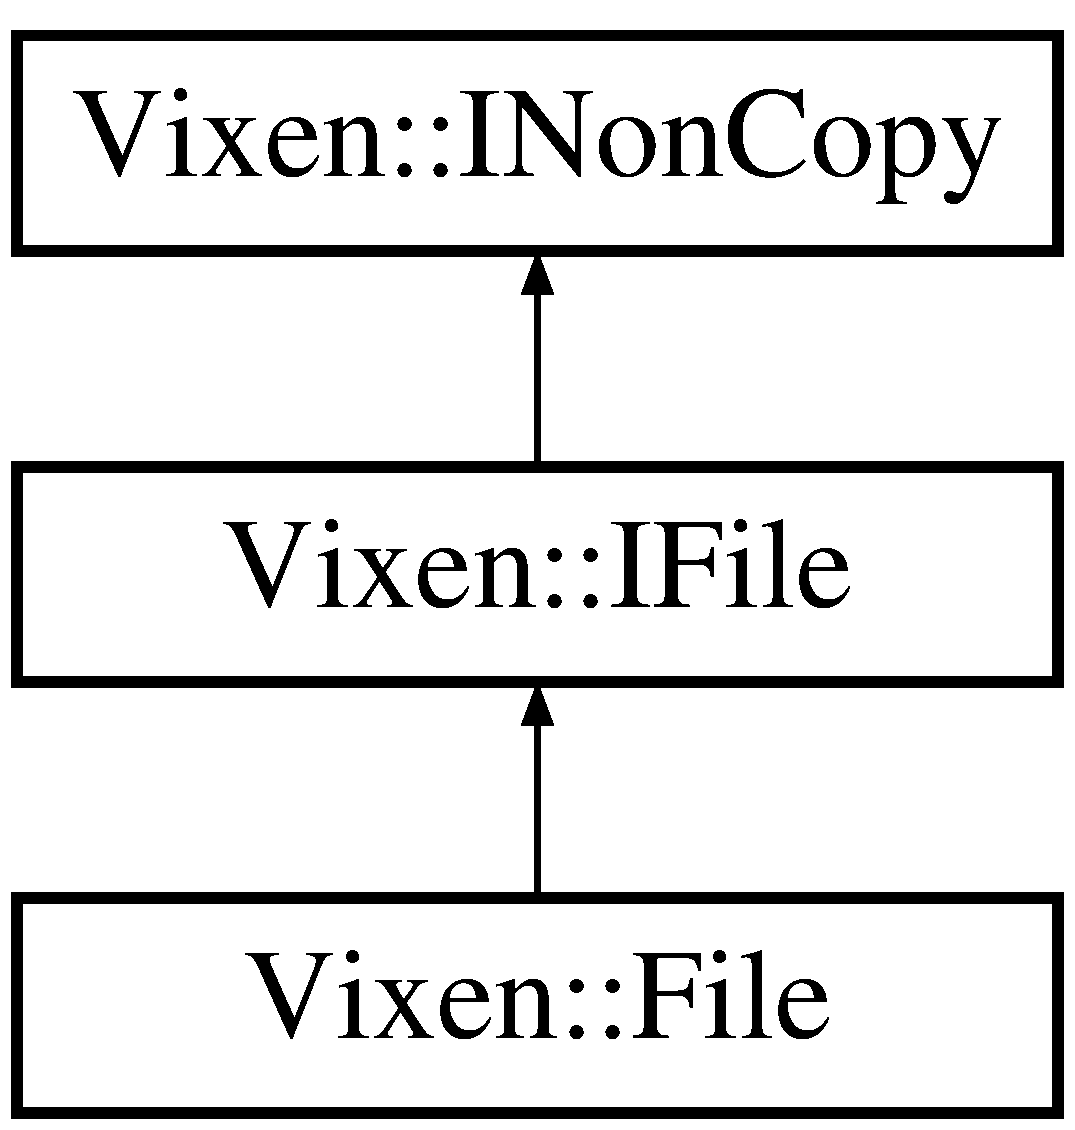
\includegraphics[height=3.000000cm]{class_vixen_1_1_file}
\end{center}
\end{figure}
\subsection*{Public Member Functions}
\begin{DoxyCompactItemize}
\item 
\hypertarget{class_vixen_1_1_file_a14ec6c12a37a1f60617bbf9313b24d8f}{}virtual File\+Error {\bfseries Error} ()\label{class_vixen_1_1_file_a14ec6c12a37a1f60617bbf9313b24d8f}

\item 
\hypertarget{class_vixen_1_1_file_a10b0b7cf7ead8a8936aa22cc1f6b9318}{}virtual U\+String {\bfseries File\+Name} ()\label{class_vixen_1_1_file_a10b0b7cf7ead8a8936aa22cc1f6b9318}

\item 
\hypertarget{class_vixen_1_1_file_a2985c6a6cb9a53f6eef0e125e6885051}{}virtual U\+String {\bfseries File\+Path} ()\label{class_vixen_1_1_file_a2985c6a6cb9a53f6eef0e125e6885051}

\item 
\hypertarget{class_vixen_1_1_file_a55e0c906130d29cf5583503016342ddd}{}virtual U\+String {\bfseries Base\+Name} ()\label{class_vixen_1_1_file_a55e0c906130d29cf5583503016342ddd}

\item 
\hypertarget{class_vixen_1_1_file_ac3869f8194a442f31d86122dfa8a3837}{}virtual bool {\bfseries Flush} ()\label{class_vixen_1_1_file_ac3869f8194a442f31d86122dfa8a3837}

\item 
\hypertarget{class_vixen_1_1_file_a24d43934cc6c607ebba11596c7429595}{}virtual bool {\bfseries Open} (U\+String path)\label{class_vixen_1_1_file_a24d43934cc6c607ebba11596c7429595}

\item 
\hypertarget{class_vixen_1_1_file_a4def6de72e2f89dc08c1cd1f0c051bad}{}virtual bool {\bfseries Seek} (size\+\_\+t offset, File\+Seek mode)\label{class_vixen_1_1_file_a4def6de72e2f89dc08c1cd1f0c051bad}

\item 
\hypertarget{class_vixen_1_1_file_ad90fede619bb354587493474f45a7bf5}{}virtual int {\bfseries Read} (B\+Y\+T\+E $\ast$out, size\+\_\+t len)\label{class_vixen_1_1_file_ad90fede619bb354587493474f45a7bf5}

\item 
\hypertarget{class_vixen_1_1_file_a3f1848aba4558bd98714c528c3fe0b73}{}virtual bool {\bfseries Close} ()\label{class_vixen_1_1_file_a3f1848aba4558bd98714c528c3fe0b73}

\item 
\hypertarget{class_vixen_1_1_file_a3071f337ce92a2a8bcb1470cabc1ca87}{}virtual size\+\_\+t {\bfseries Tell} ()\label{class_vixen_1_1_file_a3071f337ce92a2a8bcb1470cabc1ca87}

\item 
\hypertarget{class_vixen_1_1_file_a039eb93e24d180e4dd9779c9667242f0}{}virtual size\+\_\+t {\bfseries Size\+Bytes} ()\label{class_vixen_1_1_file_a039eb93e24d180e4dd9779c9667242f0}

\item 
\hypertarget{class_vixen_1_1_file_a5d5bbcc901aacfaeba1c034eedb791df}{}virtual size\+\_\+t {\bfseries Size\+K\+Bytes} ()\label{class_vixen_1_1_file_a5d5bbcc901aacfaeba1c034eedb791df}

\item 
\hypertarget{class_vixen_1_1_file_acdc342b07d6d1f7b11d5b0edcb573ddc}{}virtual size\+\_\+t {\bfseries Position} ()\label{class_vixen_1_1_file_acdc342b07d6d1f7b11d5b0edcb573ddc}

\item 
\hypertarget{class_vixen_1_1_file_a03d0e61e3fe875360cce0bdd639b2893}{}virtual F\+I\+L\+E $\ast$ {\bfseries Handle} ()\label{class_vixen_1_1_file_a03d0e61e3fe875360cce0bdd639b2893}

\item 
\hypertarget{class_vixen_1_1_file_a3d03ec3abc2fe10164dead567725fa1f}{}virtual bool {\bfseries P\+Error} (int err=0)\label{class_vixen_1_1_file_a3d03ec3abc2fe10164dead567725fa1f}

\end{DoxyCompactItemize}
\subsection*{Protected Attributes}
\begin{DoxyCompactItemize}
\item 
\hypertarget{class_vixen_1_1_file_ab696ed339a9c3f80190ab98602bbd86d}{}File\+Error {\bfseries m\+\_\+error}\label{class_vixen_1_1_file_ab696ed339a9c3f80190ab98602bbd86d}

\item 
\hypertarget{class_vixen_1_1_file_a11693f442d424e458a44b3d5d125f214}{}U\+String {\bfseries m\+\_\+file\+Path}\label{class_vixen_1_1_file_a11693f442d424e458a44b3d5d125f214}

\item 
\hypertarget{class_vixen_1_1_file_afeaa0bacfeb45b5dd635c23ed27552d9}{}U\+String {\bfseries m\+\_\+file\+Name}\label{class_vixen_1_1_file_afeaa0bacfeb45b5dd635c23ed27552d9}

\item 
\hypertarget{class_vixen_1_1_file_abb5e1d86973c517ceada94bd71a54366}{}U\+String {\bfseries m\+\_\+base\+Name}\label{class_vixen_1_1_file_abb5e1d86973c517ceada94bd71a54366}

\item 
\hypertarget{class_vixen_1_1_file_a5fe4fdd2471edc9ea7d1d0de2ad75d05}{}size\+\_\+t {\bfseries m\+\_\+position}\label{class_vixen_1_1_file_a5fe4fdd2471edc9ea7d1d0de2ad75d05}

\item 
\hypertarget{class_vixen_1_1_file_a709d76aebf0a4a81b8fb2940a52780cd}{}size\+\_\+t {\bfseries m\+\_\+size}\label{class_vixen_1_1_file_a709d76aebf0a4a81b8fb2940a52780cd}

\item 
\hypertarget{class_vixen_1_1_file_afe1a750718bfda28c1f65508cb59b187}{}F\+I\+L\+E $\ast$ {\bfseries m\+\_\+handle}\label{class_vixen_1_1_file_afe1a750718bfda28c1f65508cb59b187}

\end{DoxyCompactItemize}


The documentation for this class was generated from the following files\+:\begin{DoxyCompactItemize}
\item 
C\+:/\+Git\+Hub/\+Vixen\+Engine/include/vcore/vix\+\_\+file.\+h\item 
C\+:/\+Git\+Hub/\+Vixen\+Engine/source/vcore/vix\+\_\+file.\+cpp\end{DoxyCompactItemize}

\hypertarget{class_vixen_1_1_file_manager}{}\section{Vixen\+:\+:File\+Manager Class Reference}
\label{class_vixen_1_1_file_manager}\index{Vixen\+::\+File\+Manager@{Vixen\+::\+File\+Manager}}
Inheritance diagram for Vixen\+:\+:File\+Manager\+:\begin{figure}[H]
\begin{center}
\leavevmode
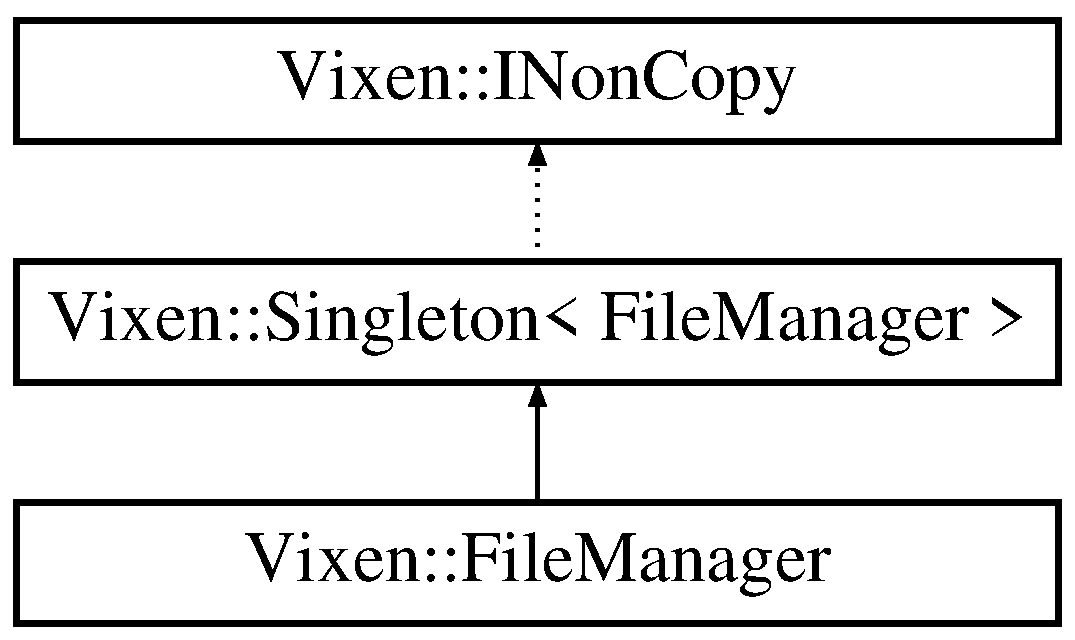
\includegraphics[height=3.000000cm]{class_vixen_1_1_file_manager}
\end{center}
\end{figure}
\subsection*{Static Public Member Functions}
\begin{DoxyCompactItemize}
\item 
\hypertarget{class_vixen_1_1_file_manager_a08c92eccb870242ecd5b3dbfb757f225}{}static void {\bfseries Initialize} ()\label{class_vixen_1_1_file_manager_a08c92eccb870242ecd5b3dbfb757f225}

\item 
\hypertarget{class_vixen_1_1_file_manager_a45f15095623024b6d6b572b5020079aa}{}static \hyperlink{class_vixen_1_1_file}{File} $\ast$ {\bfseries Open\+File} (U\+String file\+Path)\label{class_vixen_1_1_file_manager_a45f15095623024b6d6b572b5020079aa}

\item 
\hypertarget{class_vixen_1_1_file_manager_a5234580d0ccf8c9c69097ab18d7a037b}{}static void {\bfseries Close\+File} (\hyperlink{class_vixen_1_1_file}{File} $\ast$file)\label{class_vixen_1_1_file_manager_a5234580d0ccf8c9c69097ab18d7a037b}

\item 
\hypertarget{class_vixen_1_1_file_manager_a36342248ec7f83ff8917a6a210707266}{}static void {\bfseries Close\+File} (U\+String file\+Path)\label{class_vixen_1_1_file_manager_a36342248ec7f83ff8917a6a210707266}

\item 
\hypertarget{class_vixen_1_1_file_manager_a6f2939cb810556b9cc6ef63b0f7131e8}{}static \hyperlink{class_vixen_1_1_file}{File} $\ast$ {\bfseries Access\+File} (U\+String file\+Path)\label{class_vixen_1_1_file_manager_a6f2939cb810556b9cc6ef63b0f7131e8}

\item 
\hypertarget{class_vixen_1_1_file_manager_a24f3391617b3a6889edb0bf98c197411}{}static size\+\_\+t {\bfseries Total\+Files\+Open} ()\label{class_vixen_1_1_file_manager_a24f3391617b3a6889edb0bf98c197411}

\item 
\hypertarget{class_vixen_1_1_file_manager_ac7e82ebccf035b802c726ec9ccc7e813}{}static size\+\_\+t {\bfseries Total\+Bytes\+Open} ()\label{class_vixen_1_1_file_manager_ac7e82ebccf035b802c726ec9ccc7e813}

\item 
\hypertarget{class_vixen_1_1_file_manager_a07fbcfc6054fae53de098a5f123076b5}{}static void {\bfseries Print\+Open} ()\label{class_vixen_1_1_file_manager_a07fbcfc6054fae53de098a5f123076b5}

\end{DoxyCompactItemize}


The documentation for this class was generated from the following files\+:\begin{DoxyCompactItemize}
\item 
C\+:/\+Git\+Hub/\+Vixen\+Engine/include/vcore/vix\+\_\+filemanager.\+h\item 
C\+:/\+Git\+Hub/\+Vixen\+Engine/source/vcore/vix\+\_\+filemanager.\+cpp\end{DoxyCompactItemize}

\hypertarget{class_vixen_1_1_i_file}{}\section{Vixen\+:\+:I\+File Class Reference}
\label{class_vixen_1_1_i_file}\index{Vixen\+::\+I\+File@{Vixen\+::\+I\+File}}


{\ttfamily \#include $<$vix\+\_\+file\+\_\+interface.\+h$>$}

Inheritance diagram for Vixen\+:\+:I\+File\+:\begin{figure}[H]
\begin{center}
\leavevmode
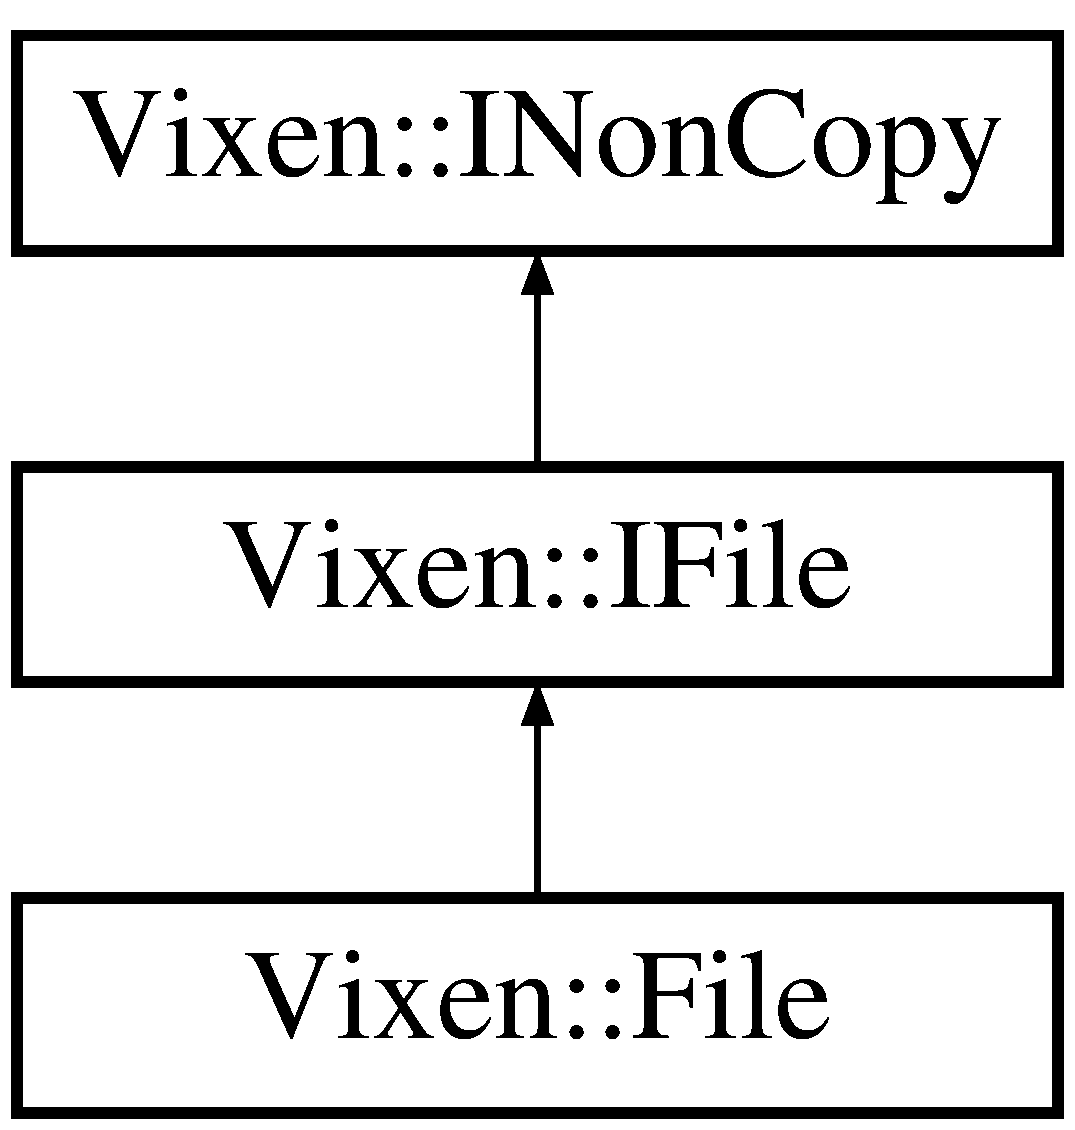
\includegraphics[height=3.000000cm]{class_vixen_1_1_i_file}
\end{center}
\end{figure}
\subsection*{Public Member Functions}
\begin{DoxyCompactItemize}
\item 
\hypertarget{class_vixen_1_1_i_file_a5918065a61d316d170d5b20f46a7a770}{}virtual File\+Error {\bfseries Error} ()=0\label{class_vixen_1_1_i_file_a5918065a61d316d170d5b20f46a7a770}

\item 
\hypertarget{class_vixen_1_1_i_file_a23244672c3e59af8dfdfd77fe6df992b}{}virtual U\+String {\bfseries File\+Name} ()=0\label{class_vixen_1_1_i_file_a23244672c3e59af8dfdfd77fe6df992b}

\item 
\hypertarget{class_vixen_1_1_i_file_aed9fd463648dbd5a5de9310711e9206b}{}virtual U\+String {\bfseries File\+Path} ()=0\label{class_vixen_1_1_i_file_aed9fd463648dbd5a5de9310711e9206b}

\item 
\hypertarget{class_vixen_1_1_i_file_a5f50dba2f5efaa1b5438b9924dad8d85}{}virtual U\+String {\bfseries Base\+Name} ()=0\label{class_vixen_1_1_i_file_a5f50dba2f5efaa1b5438b9924dad8d85}

\item 
\hypertarget{class_vixen_1_1_i_file_a719f5df723010adfcaaf2ef6fc02e414}{}virtual bool {\bfseries Open} (U\+String path)=0\label{class_vixen_1_1_i_file_a719f5df723010adfcaaf2ef6fc02e414}

\item 
\hypertarget{class_vixen_1_1_i_file_a64d455adfd53b5395ced42605aa77186}{}virtual bool {\bfseries Flush} ()=0\label{class_vixen_1_1_i_file_a64d455adfd53b5395ced42605aa77186}

\item 
\hypertarget{class_vixen_1_1_i_file_af1ebf5771acc6e8553797614de65dfd2}{}virtual bool {\bfseries Seek} (size\+\_\+t offset, File\+Seek mode)=0\label{class_vixen_1_1_i_file_af1ebf5771acc6e8553797614de65dfd2}

\item 
\hypertarget{class_vixen_1_1_i_file_ae22fba81f1a450f94bbaa993e342d28b}{}virtual bool {\bfseries Close} ()=0\label{class_vixen_1_1_i_file_ae22fba81f1a450f94bbaa993e342d28b}

\item 
\hypertarget{class_vixen_1_1_i_file_af32436aa486d7498f7fa51b7fa45b14d}{}virtual int {\bfseries Read} (B\+Y\+T\+E $\ast$out, size\+\_\+t len)=0\label{class_vixen_1_1_i_file_af32436aa486d7498f7fa51b7fa45b14d}

\item 
\hypertarget{class_vixen_1_1_i_file_a473b1cfa328219a5f85d745fe7f33ebd}{}virtual size\+\_\+t {\bfseries Tell} ()=0\label{class_vixen_1_1_i_file_a473b1cfa328219a5f85d745fe7f33ebd}

\item 
\hypertarget{class_vixen_1_1_i_file_ade8c8d3e40bebf52130c23a0bace4db8}{}virtual size\+\_\+t {\bfseries Size\+Bytes} ()=0\label{class_vixen_1_1_i_file_ade8c8d3e40bebf52130c23a0bace4db8}

\item 
\hypertarget{class_vixen_1_1_i_file_aafcb6f019831af8743e5a28fb2753126}{}virtual size\+\_\+t {\bfseries Size\+K\+Bytes} ()=0\label{class_vixen_1_1_i_file_aafcb6f019831af8743e5a28fb2753126}

\item 
\hypertarget{class_vixen_1_1_i_file_a1ca999110df6a5a71bb07f374df5f722}{}virtual size\+\_\+t {\bfseries Position} ()=0\label{class_vixen_1_1_i_file_a1ca999110df6a5a71bb07f374df5f722}

\item 
\hypertarget{class_vixen_1_1_i_file_a94e965cd24ea950f98f269317df6f010}{}virtual F\+I\+L\+E $\ast$ {\bfseries Handle} ()=0\label{class_vixen_1_1_i_file_a94e965cd24ea950f98f269317df6f010}

\item 
\hypertarget{class_vixen_1_1_i_file_aec62be3125fd105bdf059e15b4cd4603}{}virtual bool {\bfseries P\+Error} (int err=0)=0\label{class_vixen_1_1_i_file_aec62be3125fd105bdf059e15b4cd4603}

\end{DoxyCompactItemize}


\subsection{Detailed Description}
I\+F\+Ile interface

Describes base class of all \hyperlink{class_vixen_1_1_file}{File} I/\+O classes 

The documentation for this class was generated from the following file\+:\begin{DoxyCompactItemize}
\item 
C\+:/\+Git\+Hub/\+Vixen\+Engine/include/vcore/vix\+\_\+file\+\_\+interface.\+h\end{DoxyCompactItemize}

\hypertarget{class_vixen_1_1_i_manager}{}\section{Vixen\+:\+:I\+Manager Class Reference}
\label{class_vixen_1_1_i_manager}\index{Vixen\+::\+I\+Manager@{Vixen\+::\+I\+Manager}}
\subsection*{Public Member Functions}
\begin{DoxyCompactItemize}
\item 
\hypertarget{class_vixen_1_1_i_manager_add13ce871c8135673cdf607ae87ea356}{}virtual Err\+Code {\bfseries V\+Start\+Up} ()=0\label{class_vixen_1_1_i_manager_add13ce871c8135673cdf607ae87ea356}

\item 
\hypertarget{class_vixen_1_1_i_manager_a29fb4312c10a2a9e41ef455ea8d1cd6e}{}virtual Err\+Code {\bfseries V\+Shut\+Down} ()=0\label{class_vixen_1_1_i_manager_a29fb4312c10a2a9e41ef455ea8d1cd6e}

\end{DoxyCompactItemize}


The documentation for this class was generated from the following file\+:\begin{DoxyCompactItemize}
\item 
C\+:/\+Git\+Hub/\+Vixen\+Engine/include/vcore/vix\+\_\+manager.\+h\end{DoxyCompactItemize}

\hypertarget{class_vixen_1_1_i_non_copy}{}\section{Vixen\+:\+:I\+Non\+Copy Class Reference}
\label{class_vixen_1_1_i_non_copy}\index{Vixen\+::\+I\+Non\+Copy@{Vixen\+::\+I\+Non\+Copy}}
Inheritance diagram for Vixen\+:\+:I\+Non\+Copy\+:\begin{figure}[H]
\begin{center}
\leavevmode
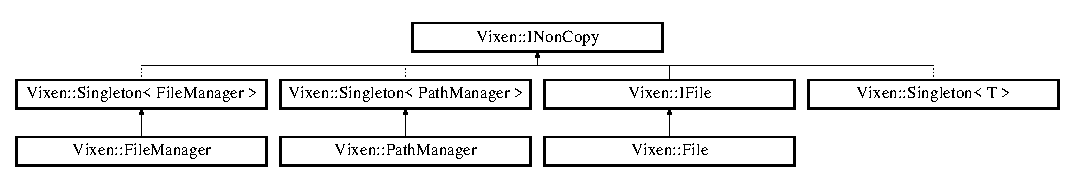
\includegraphics[height=2.000000cm]{class_vixen_1_1_i_non_copy}
\end{center}
\end{figure}


The documentation for this class was generated from the following file\+:\begin{DoxyCompactItemize}
\item 
C\+:/\+Git\+Hub/\+Vixen\+Engine/include/vcore/vix\+\_\+noncopy.\+h\end{DoxyCompactItemize}

\hypertarget{class_vixen_1_1_path_manager}{}\section{Vixen\+:\+:Path\+Manager Class Reference}
\label{class_vixen_1_1_path_manager}\index{Vixen\+::\+Path\+Manager@{Vixen\+::\+Path\+Manager}}
Inheritance diagram for Vixen\+:\+:Path\+Manager\+:\begin{figure}[H]
\begin{center}
\leavevmode
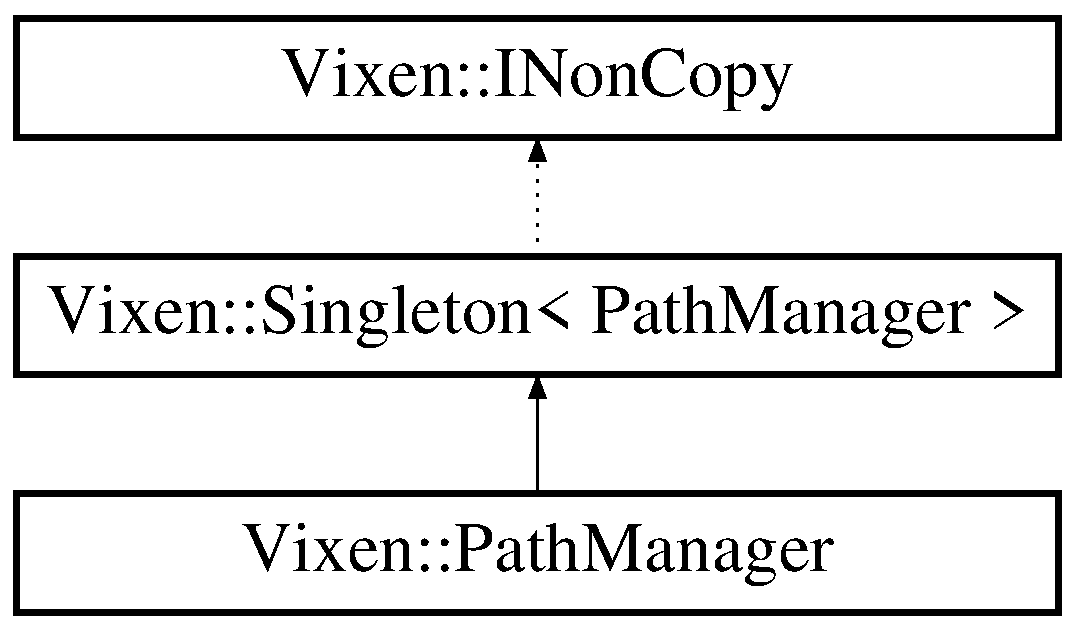
\includegraphics[height=3.000000cm]{class_vixen_1_1_path_manager}
\end{center}
\end{figure}
\subsection*{Static Public Member Functions}
\begin{DoxyCompactItemize}
\item 
\hypertarget{class_vixen_1_1_path_manager_a178ffa89f1ac1f6f5cd03f17fefea8a3}{}static void {\bfseries Initialize} ()\label{class_vixen_1_1_path_manager_a178ffa89f1ac1f6f5cd03f17fefea8a3}

\item 
\hypertarget{class_vixen_1_1_path_manager_ab4f929d54a622d0c7dfa520db9d5b2dd}{}static U\+String {\bfseries Asset\+Path} ()\label{class_vixen_1_1_path_manager_ab4f929d54a622d0c7dfa520db9d5b2dd}

\item 
\hypertarget{class_vixen_1_1_path_manager_ac860e8e2d7cea244dffcae9d6ec3ef8c}{}static U\+String {\bfseries Scene\+Path} ()\label{class_vixen_1_1_path_manager_ac860e8e2d7cea244dffcae9d6ec3ef8c}

\item 
\hypertarget{class_vixen_1_1_path_manager_a0689dea04746aeb51d25562ac32a992a}{}static U\+String {\bfseries Model\+Path} ()\label{class_vixen_1_1_path_manager_a0689dea04746aeb51d25562ac32a992a}

\item 
\hypertarget{class_vixen_1_1_path_manager_a59b6ef4d45c6355616783e8574fce25d}{}static U\+String {\bfseries Shader\+Path} ()\label{class_vixen_1_1_path_manager_a59b6ef4d45c6355616783e8574fce25d}

\item 
\hypertarget{class_vixen_1_1_path_manager_a9a09a5efd7670a09bad8c07e1be4a2b4}{}static U\+String {\bfseries Script\+Path} ()\label{class_vixen_1_1_path_manager_a9a09a5efd7670a09bad8c07e1be4a2b4}

\item 
\hypertarget{class_vixen_1_1_path_manager_a9a8b2608f60aca17401b3470b893294a}{}static U\+String {\bfseries Prefab\+Path} ()\label{class_vixen_1_1_path_manager_a9a8b2608f60aca17401b3470b893294a}

\end{DoxyCompactItemize}


The documentation for this class was generated from the following files\+:\begin{DoxyCompactItemize}
\item 
C\+:/\+Git\+Hub/\+Vixen\+Engine/include/vcore/vix\+\_\+pathmanager.\+h\item 
C\+:/\+Git\+Hub/\+Vixen\+Engine/source/vcore/vix\+\_\+pathmanager.\+cpp\end{DoxyCompactItemize}

\hypertarget{class_vixen_1_1_singleton}{}\section{Vixen\+:\+:Singleton$<$ T $>$ Class Template Reference}
\label{class_vixen_1_1_singleton}\index{Vixen\+::\+Singleton$<$ T $>$@{Vixen\+::\+Singleton$<$ T $>$}}
Inheritance diagram for Vixen\+:\+:Singleton$<$ T $>$\+:\begin{figure}[H]
\begin{center}
\leavevmode
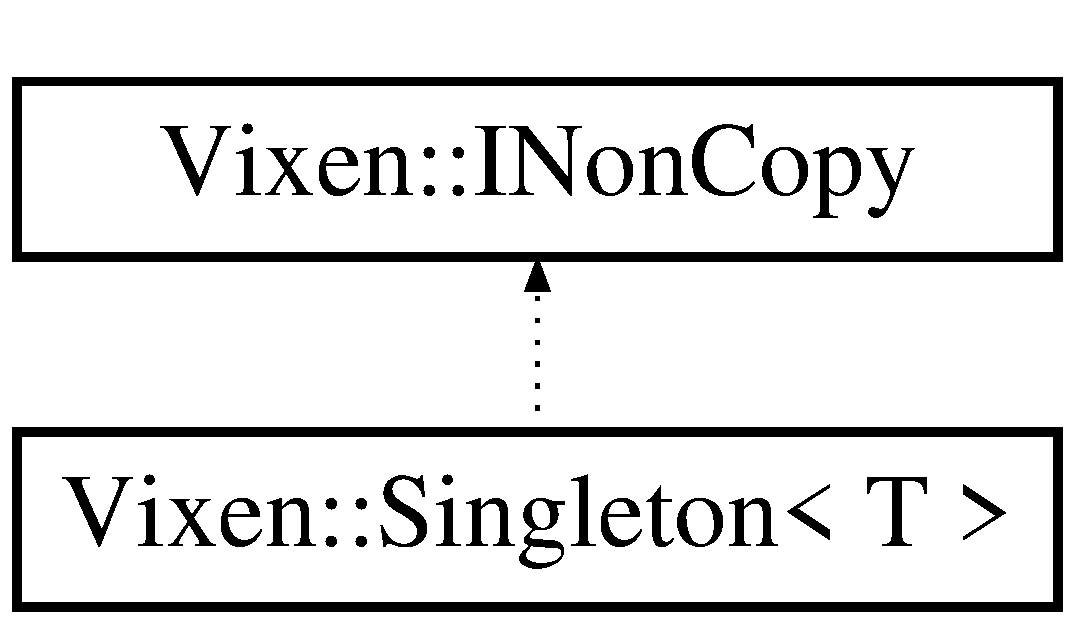
\includegraphics[height=2.000000cm]{class_vixen_1_1_singleton}
\end{center}
\end{figure}
\subsection*{Static Public Member Functions}
\begin{DoxyCompactItemize}
\item 
\hypertarget{class_vixen_1_1_singleton_a2b64eef896e902ce89a898432c0309fe}{}static T \& {\bfseries instance} ()\label{class_vixen_1_1_singleton_a2b64eef896e902ce89a898432c0309fe}

\end{DoxyCompactItemize}


The documentation for this class was generated from the following file\+:\begin{DoxyCompactItemize}
\item 
C\+:/\+Git\+Hub/\+Vixen\+Engine/include/vcore/vix\+\_\+singleton.\+h\end{DoxyCompactItemize}

%--- End generated contents ---

% Index
\backmatter
\newpage
\phantomsection
\clearemptydoublepage
\addcontentsline{toc}{chapter}{Index}
\printindex

\end{document}
